% !TEX root = master.tex
% !TEX encoding = UTF-8 Unicode

\documentclass[12pt,letterpaper]{scrbook}

\usepackage{amsmath}
\usepackage{amsthm}
\usepackage{amssymb}
\usepackage[french]{babel}
\usepackage{empheq}
\usepackage[T1]{fontenc}
\usepackage[utf8]{inputenc}
\usepackage{makeidx}     % For automatically-generated index
\usepackage{../style/leconsstyle} % Custom styles
\usepackage[]{moresize}
\usepackage{graphicx}

\theoremstyle{plain}
\newtheorem{thm}{Theorem}

\begin{document}

\author{Jean-Gaston Darboux}
\title{Leçons sur la Théories Générale Des Surfaces et les Applications Géométriques du Calcul Infinitésimal}

\clearpage
%% temporary titles
% command to provide stretchy vertical space in proportion
\newcommand\nbvspace[1][3]{\vspace*{\stretch{#1}}}
% allow some slack to avoid under/overfull boxes
\newcommand\nbstretchyspace{\spaceskip0.5em plus 0.25em minus 0.25em}
% To improve spacing on titlepages
\newcommand{\nbtitlestretch}{\spaceskip0.6em}
\pagestyle{empty}
\begin{center}
\bfseries
\nbvspace[1]
\Huge
{\huge
Leçons sur la Théorie Générale Des Surfaces}

%\nbvspace[1]
\normalsize

et les Applications Géométriques du Calcul Infinitésimal

\nbvspace[1]
\small PAR\\
\Large JEAN-GASTON DARBOUX\\[0.5em]

\nbvspace[2]

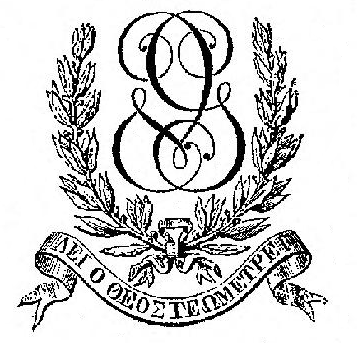
\includegraphics[width=2.5in]{../images/Logo_Gauthier-Villars.png}
\nbvspace[3]
\normalsize

PARIS\\
\large
GAUTHIER-VILLARS, IMPRIMEUR-\'EDITEUR \\
1887
\nbvspace[1]
\end{center}

\frontmatter
\tableofcontents
%%%%%%%%%% Start TeXmacs macros
\newcommand{\tmtextit}[1]{{\itshape{#1}}}
%%%%%%%%%% End TeXmacs macros

\chapter*{Préface}

L'Ouvrage dont je publie aujourd'hi la première Partie est la résumé des Leçons que j'ai faites à la Sorbonne pendant 
les hivers de 1882 à 1885. J'avais commencé l'exposition de la \textit{Théorie des surfaces} dans le but unique d'y 
trouver des applications nouvelles de la théorie, si vaste et si peu connue, des équations aux dérivées partielles. Je 
comptais consacrer une année à peine à cet enseignement; mais l'intérêt du sujet, et aussi les demandes de mes 
auditeurs, m'on entrainé bien au delà des limites que j'avais primitivement fixées.

Ce premier Volume comprend trois parties distinctes. Le premier Livre traite des \textit{Applications à la Géométries 
de la théorie des mouvements relatifs}; j'aurai à revenir sur les propositions qui y sont exposées, dans la partie où 
seront étudiées plus tard, avec tous les détails nécessaires, les belles formules de M. Codazzi. Le second Livre 
contient l'étude des \textit{différents systèmes de coordonnées curvilignes}. J'y considère successivement les systèmes 
à lignes conjuguées, dont l'étude a été trop négligée, les lignes asymptotiques, les lignes de courbure, les systèmes 
orthogonaux et isothermes.

Le Volume se termine par le \textit{Théorie des surfaces minima}, où j'ai mis à profit les travaux si remarquable 
publiés par d'éminents géometres dans ces dernières années. Elle form à peu près la moitié de ce Volume; sauf les trois 
derniers Chapitres, qui ont été rédigés au moment de l'impression, elle a été enseignée à deux reprises diffèrentes, en 
1882 et 1885. Une ou deux questions importantes y ont été omises; elles seront mieux à leur place dans la suite, quand 
j'aurai donné les propositions générales auxquelles on peut les rattacher.

Suivant son habitude constante, M. Gauthier-Villars, après avoir accueilli cet Ouvrage, a apporté tous ses soins à 
l'impression; qu'il reçoive ici mes plus vifs remercîments; je dois aussi les adresser à mes auditeurs, qui ont désiré 
voir ces Leçons publiées, et, plus particulièrement, à un de nos jeunes géomètres, M. G. Koenigs, Maître de Conférences 
à l'École Normale, qui a bien voulu m'aider dans la revision des épreuves.

\begin{flushright}
  {\small{14 juin 1887.}}
\end{flushright}


\mainmatter
% !TEX root = ../master.tex
% !TEX encoding = UTF-8 Unicode

\Chapter{Du Déplacement A Un Paramètre}{Application A La Théorie Des Courbes Gauches}
\label{chp1}

\textbf{1.} Considérons un corps solide ou système invariable, mobile autour d'un point fixe. On sait qu'à un instant 
quelconque les vitesses des différents points du système sont les mêmes que s'il tournait autour d'une droite passant 
par le point fixe, droite qui a reçu le nom d'\textit{axe instantané de rotation}. On démontre en Mécanique que les 
rotations peuvent être représentées géométriquement par des droites, comme les forces, et composées ou décomposées 
suivant la même loi, c'est-a-dire que, si l'on compose ou si l'on décompose les rotations comme les forces, la vitesse 
imprimée par la rotation résultante à un point quelconque est la résultante des vitesses qui seraient communiquées au 
même point par chacune des rotations composantes, existant isolément. On sait aussi que, si l'on considère un point 
mobile par rapport au système invariable, la vitesse absolue de ce point est la résultante de sa vitesse relative et 
de sa vitesse d'\textit{entraînement}. On désigne sous ce nom la vitesse qu'aurait un point qui, à l'instant considéré, 
coïnciderait avec le point mobile, mais demeurerait invariablement lié au système solide.

Il résulte de ces propositions qu'on pourra construire, à un instant quelconque, les vitesses de tous les points du 
système invariable dès qu'on aura, en grandeur et en direction, la rotation à cet instant. Il semblerait naturel de 
déterminer à chaque instant cette rotation par ses composantes relatives à trois axes rectangulaires, fixes dans 
l'espace et ayant pour origine le point fixe du système solide. En réalité, les éléments les plus importants, les seuls 
qui permettent le plus souvent une étude approfondie due mouvement, ce sont les composantes de la rotation relativement 
à des axes mobiles, entraînés dans le mouvement du système invariable. Rappelons rapidement la méthode employée en 
Mécanique.

Soient $OX$, $OY$, $OZ$ trois axes fixes passant par le point fixe $O$ du système et $Ox$, $Oy$, $Oz$ trois axes 
rectangulaires invariablement liés au système mobile. Nous supposerons que les deux systèmes d'axes aient la mêmes 
disposition, c'est-à-dire qu'ils puissent être amenés à coïncider. De plus, nous supposerons que les sens des axes 
aient été choisis de telle manière que la rotation autour de $OZ$, qui déplacerait $OX$ du côté de $OY$, soit 
représentée par une droite dirigée suivant la partie positive de OZ. Nous déterminerons les axes mobiles par les 
cosinus des angles qu'ils forment avec les axes fixes. Pour cela nous écrirons le Tableau 

\begin{center}
	\bgroup
	\def\arraystretch{1.7}
	%\setlength\tabcolsep{10.7pt}
	\begin{tabular}{ |c|c|c|c| } 
	\hline
	 & $x$ & $y$ & $z$ \\
	\hline
	$X$ & $a$ & $b$ & $c$ \\
	\hline
	$Y$ & $a'$ & $b'$ & $c'$ \\ 
	\hline
	$Z$ & $a''$ & $b''$ & $c''$ \\
	\hline
	\end{tabular}
	\egroup
\end{center}
qui fait connaître les cosinus des angles formés par chacun des axes fixes avec les axes mobiles. 

On a les relations
\begin{empheq}[left=\empheqlbrace]{equation}
	\begin{aligned}
        & a^2 + b^2 + c^2 = 1,    \quad && aa' + bb' + cc' = 0, \\
        & a^2 + a'^2 + a''^2 = 1, \quad && ab + a'b' + a''c'' = 0, \\
        & a = b'c'' - c'b'',      \quad && \begin{vmatrix} a & b & c \\ a' & b' & c' \\ a'' & b'' & c'' \end{vmatrix} = 1,
	\end{aligned} \label{eqn-1}
\end{empheq}
auxquelles il faut joindre toutes celles que l'on obtiendrait par des permutations circulaires effectuées, soit sur les lettres, soit sur les indices. Rappelons encore que les neuf cosinus peuvent être exprimés par les trois angles d'Euler, au moyen des formules
\begin{empheq}[left=\empheqlbrace]{equation}
	\begin{aligned}
        a   &= \cos\theta \sin\varphi \sin\psi + \cos\varphi \cos\psi, \\
        b   &= \cos\theta \sin\psi \cos\varphi - \cos\psi \sin\varphi, \\
        c   &= \sin\theta \sin\psi \\
        a'  &= \cos\theta \cos\psi \sin\varphi - \sin\psi \cos\varphi, \\
        b'  &= \cos\theta \cos\psi \cos\varphi + \sin\psi \sin\varphi, \\
        c'  &= \sin\theta \cos\psi, \\
        a'' &= -\sin\theta \sin\varphi, \\
        b'' &= -\sin\theta \cos\varphi, \\
        c'' &= \cos\phi.
	\end{aligned} \label{eqn-2}
\end{empheq}
Désignons maintenant par $p$, $q$, $r$ les composantes de la rotation à l'instant $t$ par rapport aux axes mobiles. 
Considérons un point dont les coordonnées soient $x$, $y$, $z$, relativement aux axes mobiles, et cherchons les 
composantes de sa vitesse absolue par rapport aux mêmes axes. En écrivant que cette vitesse absolue est la résultante
de la vitesse relative et de celles qui seraient dues aux trois rotations $p$, $q$, $r$, on obtiendra les expressions
suivantes de ces composantes
\begin{empheq}[left=\empheqlbrace]{equation}
	\begin{aligned}
        V_x &= \frac{\d{x}}{\d{t}} + qx - ry, \\
        V_y &= \frac{\d{y}}{\d{t}} + rx - pz, \\
        V_z &= \frac{\d{z}}{\d{t}} + py - qx,
	\end{aligned} \label{eqn-1.3}
\end{empheq}
dont nous aurons souvent à faire usage.

Nous allons montrer, dès à présent, comment on peut en déduire les expressions de $p$, $q$, $r$ en fonction des neuf 
cosinus et de leurs dérivées par rapport au temps. Pour cela, considérons le point pris sur l'axe $OX$ à la distance 
$1$. Ce point a pour coordonnées relatives (c'est-à-dire relativement aux axes mobiles) $a$, $b$, $c$. En exprimant que 
sa vitesse est nulle et en appliquant les formules \ref{eqn-1.3}, nous obtiendrons les équations fondamentales
\begin{empheq}[left=\empheqlbrace]{equation}
	\begin{aligned}
		\frac{\d{a}}{\d{t}} &= br - cq, \\
		\frac{\d{b}}{\d{t}} &= cp - ar, \\
		\frac{\d{c}}{\d{t}} &= aq - bp,
	\end{aligned} \label{eqn-1.4}
\end{empheq}
auxquelles on peut joindre les suivantes
\begin{empheq}[left=\empheqlbrace]{equation}
	\begin{aligned}
		\frac{\d{a'}}{\d{t}} &= b'r - c'q, \\
		\frac{\d{b'}}{\d{t}} &= c'p - a'r, \\
		\frac{\d{c'}}{\d{t}} &= a'q - b'p;
	\end{aligned} \label{eqn-1.4p}
\end{empheq}
\begin{empheq}[left=\empheqlbrace]{equation}
	\begin{aligned}
		\frac{\d{a''}}{\d{t}} &= b''r - c''q, \\
		\frac{\d{b''}}{\d{t}} &= c''p - a''r, \\
		\frac{\d{c''}}{\d{t}} &= a''q - b''p,
	\end{aligned} \label{eqn-1.4pp}
\end{empheq}
que l'on démontrera de la même manière.

On déduit de là les formules
\begin{empheq}[left=\empheqlbrace]{equation}
	\begin{aligned}
		p \d{t} &= \sum{c}\d{b} = - \sum{b} \d{c}, \\
		q \d{t} &= \sum{a}\d{c} = - \sum{c} \d{a}, \\
		r \d{t} &= \sum{b}\d{a} = - \sum{a} \d{b},
	\end{aligned} \label{eqn-1.5}
\end{empheq}
qui donnent les valeurs cherchées des rotations. Si l'on remplace les cosinus par leurs expressions en fonction des 
angles d'Euler, on aura le système
\begin{empheq}[left=\empheqlbrace]{equation}
	\begin{aligned}
		p &= \sin\varphi\sin\theta\frac{\d{\psi}}{\d{t}} - \cos\varphi\frac{\d{\theta}}{\d{t}}, \\
		q &= \cos\varphi\sin\theta\frac{\d{\psi}}{\d{t}} + \sin\varphi\frac{\d{\theta}}{\d{t}}, \\
		r &= \frac{\d{\varphi}}{\d{t}} - \cos\theta\frac{\d{\psi}}{\d{t}},
	\end{aligned} \label{eqn-1.6}
\end{empheq}
qu'il serait aisé de démontrer géométriquement. En résolvent par rapport aux dérivées des angles, on trouve
\begin{empheq}[left=\empheqlbrace]{equation}
	\begin{aligned}
		\frac{\d\theta}{\d{t}} &= q\sin\varphi - p\cos\varphi, \\
		\sin\theta\frac{\d\psi}{\d{t}} &= q\cos\varphi + p\sin\varphi, \\
		\frac{\d\varphi}{\d{t}} &= r + \cot\theta(p\sin\varphi + q\cos\varphi).
	\end{aligned} \label{eqn-1.7}
\end{empheq}

\textbf{2.} Tout cela étant rappelé, nous allons étudier la question suivante, qui est fondamentale dans notre théorie: 
\textit{On donne $p$, $q$, $r$ en fonction du temps $t$, et l'on propose de déterminer complètement le mouvement.}

Il est clair que la question sera résolue si l'on a les expressions des neuf cosinus en fonction du temps. Or il 
résulte immédiatement des formules \ref{eqn-1.4} que, si l'on sépare les cosinus en trois groupes, formés 
respectivement de $a$, $b$, $c$; $a'$, $b'$, $c'$; $a''$, $b''$, $c''$, les trois cosinus de chaque groupe sont des  
solutions simultanées du système
\begin{empheq}[left=\empheqlbrace]{equation}
	\begin{aligned}
		\frac{\d\alpha}{\d{t}} &= \beta r - \gamma q, \\
		\frac{\d\beta}{\d{t}} &= \gamma p - \alpha r, \\
		\frac{\d\gamma}{\d{t}} &= \alpha q - \beta p. \\
	\end{aligned} \label{eqn-1.8}
\end{empheq}

Toute la difficulté se réduit donc à l'intégration de ce système. L'étude détaillée de cette intégration fera l'objet 
du Chapitre suivant. Pour le moment nous nous contenterons de signaler les propriétés suivantes du système 
\ref{eqn-1.8}.

D'abord, par suite de sa forme linéaire, il admettra toujours une solution, et une seule, pour laquelle les valeurs 
initiales de $\alpha$, $\beta$, $\gamma$ seront données.

En second lieu, si $\alpha$, $\beta$, $\gamma$; $\alpha'$, $\beta'$, $\gamma'$ désignent deux systèmes de solutions 
quelconques, les expressions
\[
	\alpha^2 + \beta^2 + \gamma^2,
	 \quad \alpha\alpha' + \beta\beta' + \gamma\gamma',
	 \quad \alpha'^2 + \beta'^2 + \gamma'^2
\]
seront des constantes. On le reconnaît aisément en les différentiant et tenant compte des équations \ref{eqn-1.8}.

Ces propriétés vont nous permettre d'établir qu'il y a toujours, quelles que soient	les expressions de $p$, $q$, $r$ en 
fonction du temps, une infinité de mouvements dans lesquels ces trois quantités sont les composantes de la rotation 
relativement aux axes mobiles.

Considérons en effet un trièdre trirectangle $(T_0)$, de même sens que le trièdre $OXYZ$, formé par les axes fixes et 
soient $a_0$, $b_0$, $c_0$, \ldots les cosinus directeurs de $OX$, $OY$, $OZ$ par rapport aux axes de $(T_0)$. 
Déterminons les trois systèmes de solutions des équations \ref{eqn-1.8}, $a$, $b$, $c$; $a'$, $b'$, $c'$; $a''$, $b''$, 
$c''$, qui correspondent respectivement aux valeurs initiales suivantes: $a_0$, $b_0$, $c_0$; $a'_0$, $b'_0$, $c'_0$; 
$a''_0$, $b''_0$, $c''_0$.

Les fonctionnes, telles que
\[
	a^2 + b^2 + c^2, \quad aa' + bb' + cc', \ldots,
\]
ayant pour valeur initiale 1 ou 0, et devant rester constantes d'après les propriétés du système (\ref{eqn-1.8}), ne 
cesseront pas de conserver leurs valeurs initiales; par conséquent, les neufs quantités $a$, $a'$, $a''$, \ldots seront 
à chaque instant les cosinus directeurs de trois droites rectangulaires formant un trièdre mobile $(T)$ dont la 
position initiale sera $(T_0)$. Comme cette position initiale peut être choisi à volonté, on voit qu'il existe une 
infinité de mouvements pour lesquels $p$, $q$, $r$ sont des fonctions données du temps.

Tous ces mouvements, qui dépendent de trois constantes arbitraires, se réduisent au fond à un seul, mais qui serait 
rapporté à des axes fixes différents.

En effet, considérons, dans l'un quelconque d'entre eux, la position occupé par le trièdre mobile à l'instant initial, 
et choisissons-la pour le système d'axes fixes auquel nous rapporterons le mouvement du système mobile. Les valeurs 
initiale des neufs cosinus sont alors 1 ou 0, la solution qui correspond à ces valeurs numériques ne contient aucune 
constante arbitraire et est bien déterminée.

Il résulte de ce qui précède que, lorsqu'on aura obtenu une solution quelconque du problème, c'est-a-dire un système de 
valeurs des neufs cosinus, il suffira, si l'on veut avoir la solution la plus générale, de changer d'axes fixes, ce qui 
introduira trois constantes; puis de supposer que les nouvelles formules se rapportent aux anciens axes.

\textbf{3.} Nous allons maintenant étudier le cas où le système mobile n'a plus de point fixe. Alors il faut joindre 
aux composantes $p$, $q$, $r$ celles de la vitesse de l'origine $O$ des axes mobiles, prises toujours relativement aux 
axes mobiles $Ox$, $Oy$, $Oz$. Désignons-les par $\xi$, $\eta$, $\zeta$; jointes aux trois rotations, elles 
interviennent dans toutes les questions relatives à l'étude du mouvement. Supposons que l'on connaisse les expressions 
de ces six quantités en fonction du temps, et cherchons comment on déterminera le mouvement du trièdre mobile. 
Désignons par $(T)$ ce trièdre mobile, et soit $(T')$ le trièdre dont l'origine est un point fixe quelconque et dont 
les axes sont parallèles à ceux de $(T)$. A un instant quelconque les deux trièdres sont animés de la même rotation et, 
par conséquent, les neufs cosinus se détermineront au moyen de $p$, $q$, $r$ comme dans le cas précédent; d'ailleurs, 
si $X_0$, $Y_0$, $Z_0$ désignent les coordonnées de l'origine mobile $O$ par rapport aux axes fixes, on a évidemment, 
en projetant la vitesse de cette origine sur les axes fixes,
\begin{empheq}[left=\empheqlbrace]{equation}
	\begin{aligned}
		\frac{\d{X_0}}{\d{t}} &= a\xi + b\eta + c\zeta, \\
		\frac{\d{Y_0}}{\d{t}} &= a'\xi + b'\eta + c'\zeta, \\
		\frac{\d{Z_0}}{\d{t}} &= a''\xi + b''\eta + c''\zeta.
	\end{aligned} \label{eqn-1.9}
\end{empheq}

Quand on aura déterminé les cosinus, ces formules feront connaître $X_0$, $Y_0$, $Z_0$ par de simples quadratures qui 
introduiront trois constantes nouvelles.

Ici encore, tous les mouvements possibles correspondants aux différents valeurs des six constantes arbitraires se 
réduisent à un seul et même mouvement, observé par rapport à des axes différents; car l'intégration n'introduit aucune 
constante arbitraire et ne donne qu'un seul mouvement, si l'on suppose que les axes fixes coïncident avec la position 
initiale des axes mobiles.

Je rappellerai, relativement au cas que nous venons de considérer, que si $x$, $y$, $z$ sont les coordonnées d'un point 
relativement aux axes mobiles, la vitesse absolue de ce point aura pour composantes, relatives aux mêmes axes, les 
trois quantités 
\begin{empheq}[left=\empheqlbrace]{equation}
	\begin{aligned}
		V_x = \xi + qz - ry + \frac{\d{x}}{\d{t}}, \\
		V_y = \eta + rx - pz + \frac{\d{y}}{\d{t}}, \\
		V_z = \zeta + py - qx + \frac{\d{z}}{\d{t}}.
	\end{aligned} \label{eqn-1.10}
\end{empheq}

Considérons, par exemple, les points invariablement liés au système mobile et cherchons ceux pour lesquels la vitesse 
est minimum. Il faudra déterminer les valeurs de $x$, $y$, $z$ rendant minimum la somme
\[
	(\xi + qx - ry)^2 + (\eta + rx - pz)^2 + (\zeta + py -qx)^2.
\]

En égalant à zéro les dérivées par rapport à $x$, à $y$ et à $z$, on obtient trois équations qui se réduisent aux deux 
suivantes:
\[
	\frac{\xi + qz - ry}{p} = \frac{\eta + rx - pz}{q} = \frac{\zeta + py - qx}{r}.
\]

Ces deux équations représentent une droite, l'axe central du mouvement à l'instant considéré. On trouve facilement, 
pour la valeur commune des rapports précédents,
\[
	\frac{\xi p + \eta q + \zeta r}{p^2 + q^2 + r^2},
\]
ce qui donne, pour la valeur minimum de la vitesse,
\[
	\frac{\xi p + \eta q + \zeta r}{\sqrt{p^2 + q^2 + r^2}}.
\]

La condition nécessaire et suffisante pour que le mouvement du système se réduise à une simple rotation est done la 
suivant
\[
	\xi p + \eta q + \zeta r = 0,
\]
et, dans ce cas, l'axe de rotation est représenté par les trois équations
\begin{empheq}[left=\empheqlbrace]{equation}
	\begin{aligned}
		\xi + qx - ry &= 0, \\
		\eta + rx - pz &= 0, \\
		\zeta + py - qx &= 0,
	\end{aligned} \label{eqn-1.11}
\end{empheq}
qui caractérisent en effet les points dont la vitesse est nulle, comme le montrent les formules (\ref{eqn-1.10}).

\textbf{4.} Pour indiquer dès à présent une application des propositions précédentes, considérons une courbe gauche 
quelconque et étudions le mouvement du trièdre $(T)$ formé par la tangente que nous prendrons pour axe des $x$, la 
normale principale que nous prendrons pour axe des $y$, en la supposant, par exemple, dirigée vers la centre de 
courbure, et la binormale qui sera l'axe des $z$ et dont le sens est défini par les conventions déjà faites.

Prenons l'arc $s$ comme variable indépendante ou, ce qui est la même chose, supposons
\[
	\frac{\d{s}}{\d{t}} = 1.
\]

On a ici,
\[
	\xi = 1, \quad \eta = 0, \quad \zeta = 0,
\]
et, si $x$, $y$, $z$ désignent les coordonnées du pointe de la courbe, qui est le sommet du trièdre, par rapport à des 
axe fixes,
\[
	a = \frac{\d{x}}{\d{s}}, \quad a' = \frac{\d{y}}{\d{s}}, \quad a'' = \frac{\d{z}}{\d{t}}.
\]

Les formules générales (\ref{eqn-1.4}) nous donnent
\begin{equation}
	\d{a} = (br - cq)\d{s}, \quad \d{b} = (cp - ar)\d{s}, \quad dc = (aq - bp)\d{s}.
	\label{eqn-1.12}
\end{equation}

Exprimons que la binormale, dont les cosinus directeurs sont $c$, $c'$, $c''$, est perpendiculaire au plan osculateur, 
c'est-à-dire aux deux droites dont les cosinus directeurs sont $a$, $a'$, $a''$ et $a + \d{a}$, $a' + \d{a'}$, $a'' + 
\d{a''}$. L'une des équations sera satisfaite d'elle-même et l'autre nous donnera la condition
\[
	\sum{c}\d{a} = q \d{s} = 0.
\]

Ainsi la composante $q$ doit être nulle, et les formules (\ref{eqn-1.12}) se réduisent aux suivantes:
\begin{equation}
	\frac{\d{a}}{\d{s}} = br, \quad \frac{\d{b}}{\d{s}} = cp - ar, \quad \frac{\d{c}}{\d{s}} = - bp
	\label{eqn-1.13}
\end{equation}
Il est aisé d'obtenir la signification géométrique des rotations $p$ et $r$.

Menons en effet par un point fixe des parallèles aux arêtes du trièdre $(T)$; nous obtiendrons un trièdre $(T_1)$ dont 
la rotation sera la même, à un instant quelconque, que celle du trièdre $(T)$. Un point situé à la distance 1 sur l'axe 
de $x$ du trièdre $(T_1)$ aura une vitesse dont les composantes seront, d'après les formules (\ref{eqn-1.3}),
\[
	0, \quad r, \quad 0,
\]
et, par conséquent, ce point décrira le chemin $r \d{s}$; ou, ce qui est la même chose, la tangente à la courbe 
tournera de l'angle $r \d{s}$ quand son point de contact décrira l'arc $\d{s}$; donc la composante $r$ est égale à la 
première courbure de la courbe.

En prenant un point situé à la distance 1 sur l'axe des $z$ du trièdre $(T_1)$, on verra de même que les composantes de 
sa vitesse seront
\[
	0, \quad -p, \quad 0,
\]
et, par conséquent, le plan osculateur tournera de l'angle $-p \d{s}$, quand le point de la courbe décrira l'arc 
$\d{s}$. En d'autres termes, $-p$ sera la torsion de la courbe. Ainsi nous pourrons poser
\begin{equation}
	r = \frac{1}{\rho},\quad p = -\frac{1}{\tau},
	\label{eqn-1.14}
\end{equation}
$\rho$ et $\tau$ désignant les rayons de courbure et de torsion, et les formules (\ref{eqn-1.13}) deviendront
\begin{equation}
	\frac{\d{a}}{\d{s}} = \frac{b}{\rho}, 
	 \quad \frac{\d{c}}{\d{s}} = \frac{b}{\tau},
	 \quad \frac{\d{b}}{\d{s}} = - \frac{c}{\tau} - \frac{a}{\rho}.
	\label{eqn-1.15}
\end{equation}

On reconnaît les formules de J.-A. Serret, qui jouent un rôle si important dans la théorie des courbes gauches.

\textbf{5.} La méthode qui nous a permis de les établir met en évidence quelques propositions qu'il serait aisé de 
démontrer autrement et dont on fait un usage continuel dans les démonstrations géométriques.

Étant donnée la courbe gauche $(C)$, si par l'origine on mène une parallèle à la tangente de cette courbe, de longueur 
égale à 1, l'extrémité de cette parallèle décrira une courbe sphérique que nous appellerons, avec M. P. Serret, 
l'\textit{indicatrice sphérique} de la courbe gauche. Il résulte de ce qui précède que la tangente à l'indicatrice 
sphérique est parallèle à la normale principale de la courbe $(C)$; car le point qui décrit l'indicatrice est celui qui 
est situé à la distance 1 sur l'axe des $x$ du trièdre $(T_1)$, et nous avons vu que la vitesse de ce point est égale à 
$\frac1\rho$ et parallèle à la normale principale. 

De même, si par l'origine nous menons une droite de longueur 1, parallèle à la binormale, l'extrémité de cette droite 
sera le point à la distance 1 sur l'axe des $z$ du trièdre $(T_1)$; ce point aura une vitesse égale à $\frac1\tau$ et 
qui sera encore parallèle à la normale principale; la courbe sphérique qu'il décrit sera parallèle à l'indicatrice: on 
l'obtiendra en portant sur les grands cercles normaux à l'indicatrice, et dans un sens convenable, une longueur égale à 
un quadrant; en d'autres termes, ce sera la \textit{courbe polaire} de l'indicatrice sphérique.

\textbf{6.} Nous signalerons encore la théorème suivant qui est fort important:
\begin{theorem}
	Toute courbe, dans laquelle le rapport $\frac\rho\tau$ est constant, est une hélice tracée sur un cylindre 
	quelconque.
\end{theorem}

En effet, si nous considérons le mouvement de trièdre $(T_1)$ parallèle à $(T)$, nous avons que, la composante $q$ 
étant nulle, l'axe instantané de rotation est toujours dans le plan des $xz$. Lorsque le rapport $\frac\rho\tau$ ou 
$\frac{-p}{r}$ demeurera constant, cet axe instantané deviendra fixe par rapport aux axes mobiles. Or on sait que, 
lorsque l'axe instantané occupe une position invariable par rapport au système mobile, il demeure fixe dans l'espace. 
Le trièdre $(T_1)$ tournera donc autour d'une droite fixe; son axe des $x$, qui est parallèle à la tangente de la 
courbe, fera un angle constante avec cette droite fixe et engendrera un cône de révolution. On reconnaît la propriété 
caractéristique de l'hélice tracée sur un cylindre quelconque.

Lorsque $\rho$ et $\tau$ sont constants, cette hélice est tracée sur un cylindre de révolution. Dans ce cas, en effet, 
le mouvement du trièdre $(T)$ présente à chaque instant un translation et un rotation invariables. Alors tous les 
points du système mobile, et en particulaire l'origine du trièdre, décrivent des hélices tracées sur des cylindres 
circulaires droits.

\textbf{7.} Dans le mouvement que nous venons d'étudier, trois des six quantités $\xi$, \ldots, $p$, \ldots sont 
nulles. Nous allons montrer que, réciproquement, si l'on a
\[
	\eta = \zeta = q = 0,
\]
l'origine du trièdre décrit une courbe qui est tangente à l'axe des $x$ de ce trièdre et admet l'axe des $y$ pour 
normale principale. Le première point résulte immédiatement des équations
\[
	\eta = \zeta = 0.
\]

D'autre part, la composante $q$ étant nulle, nous avons
\[
	\sum{c \d{a}} = 0.
\]

L'axe des $z$ du trièdre mobile est donc normal à deux positions consécutives de l'axe des $x$. En d'autres termes, le 
plan des $xy$ est le plan osculateur de la courbe décrit par l'origine des coordonnées.

En réduisent toutes les vitesses dans le même rapport, de manière de $\xi$ devienne égale à 1, on doit remplacer $p$, 
$r$ par $\frac{p}{\xi}$, $\frac{r}{\xi}$. La courbure et la torsion de la courbe sont données par les formules
\begin{equation}
	\frac{1}{\rho} = \frac{r}{\xi}, \quad \frac{1}{\tau} = \frac{-p}{\xi}.
	\label{eqn-1.16}
\end{equation}

\textbf{8.} La méthode cinématique que nous venons d'exposer s'applique d'une manière élégante à la solution complète 
du problème suivant, complètement résolu par M. Bertrand: \textit{Rechercher s'il existe une courbe dont les normales 
principales soient aussi normales principales d'une autre courbe.}

Soient $M$ un point de la courbe donnée et $(T)$ le trièdre relatif à ce point. Si l'on porte sur la normale principale 
une longueur $MM'=a$, la vitesse du point $M'$ aura pour composantes
\[
	1 - ra, \quad \frac{\d{a}}{\d{s}}, \quad pa,
\]
suivant $Mx$, $My$, $Mz$ respectivement; cela résulte des formules (\ref{eqn-1.10}). Si l'on veut que la courbe décrite 
par le point $M'$ soit normale a $MM'$, il faudra que l'on ait
\[
	\frac{\d{a}}{\d{s}} = 0,
\]
$a$ devra être constante: ce résultat était évident \textit{a priori}, et nous aurions pu le supposer immédiatement.

Alors la vitesse $\nu$ de $M'$ est perpendiculaire à $My$ et, si l'on appelle $\omega$ l'angle qu'elle fait avec $Mx$, 
on a
\begin{empheq}[left=\empheqlbrace]{equation}
	\begin{aligned}
		\nu \cos\omega &= 1 - ra, \\
		\nu \sin\omega &= pa.
	\end{aligned} \label{eqn-1.17}
\end{empheq}

La droite $M'M$ sera alors normale de la courbe décrite par le point $M'$; mais elle ne sera pas en général normale 
principale. Construisons le trièdre $(T')$ formé par la tangente $M'x'$ à la courbe décrit par le point $M'$, par la 
droite $M'y$ et par la perpendiculaire commune à ces deux droites, et remarquons que l'axe des $y$ de ce trièdre 
coïncide avec l'axe de même nom de $(T)$. On aurait un trièdre ayant même orientation que $(T')$ en faisant tourner le 
trièdre $(T)$ de l'angle $\omega$ autour de son axe des $y$. On obtiendra donc la rotation instantanée du trièdre 
$(T')$ en composant les deux rotations $p$, $r$ du trièdre $(T)$ avec une rotation $\frac{\d{\omega}}{\d{t}}$ autour de 
$My$.

Or la condition nécessaire et suffisante pour que la droite $My$ ou $M'y$ soit la normale principale de la courbe 
décrit par le point $M'$ est, nous l'avons vu, que la rotation de $(T')$ autour de $M'y$ soit nulle. Il faudra donc que 
l'on ait
\[
	\frac{\d{\omega}}{\d{t}} = 0
\]
et, par suite, que l'angle $\omega$ soit constant. Ainsi \textit{les plans osculateurs des courbes décrites par les 
points $M$, $M'$ devront se couper sous un angle constant $\omega$}.

Si l'on se reporte maintenant aux formules (\ref{eqn-1.17}), on en déduit, par l'élimination de $\nu$,
\[
	\frac{\sin{\omega}}{a} = r \sin\omega + p \cos\omega
\]
ou, en remplaçant $r$ et $p$ par leurs expressions géométriques,
\begin{equation}
	\frac{\sin{\omega}}{a} = \frac{\sin{\omega}}{\rho} - \frac{\cos{\omega}}{\tau}.
	\label{eqn-1.18}
\end{equation}

\textit{Il y a donc une relation linéaire entre les deux courbures}.

\textbf{9.} Réciproquement, s'il existe une relation linéaire entre les deux courbures
\[
	C = \frac{A}{\rho} + \frac{B}{\tau},
\]
la courbe jouira en général de la propriété indiquée. On identifiera la relation précédente avec l'équation 
(\ref{eqn-1.18}), et l'on aura
\[
	a = \frac{A}{C}, \quad \cot{\omega} = -\frac{B}{A}.
\]
Signalons cependant deux cas d'exception:

Si l'on a $C=0$, sans que $A$ soit nul, la relation entre les courbures prend la forme
\[
	\frac{\rho}{\tau} = \textrm{const.},
\]
et $a$ devient infini. Ainsi la seconde courbe, lieu de $M'$, est rejetée à l'infini. La courbe proposée est alors une 
hélice.

Si l'on $A=0$, c'est-à-dire si la courbe a une torsion constante, $a$ est nul et les deux courbes, lieux de $M$ et 
$M'$, se confondent.

On peut avoir plus de deux courbes ayant les mêmes normales principales: $1^\circ$ si la valeur de $a$ est 
indéterminée, c'est-à-dire si l'on a $A=C=0$; dans ce cas, la courbe sera plane; $2^\circ$ s'il y a plus d'une relation 
linéaire entre les courbures, c'est-à-dire si les deux courbures sont constantes; dans ce cas, l'équation 
(\ref{eqn-1.18}) sera satisfaite pour toute valeur de $a$ et fera connaître $\omega$; il y aura donc un infinité de 
courbes ayant les mêmes normales principales. La courbe primitive et, par conséquent, toutes les autres seront des 
hélices tracées sur des cylindres circulaires droits; la surface formée par les normales principales sera l'hélicoïde 
gauche à plan directeur.

\textbf{10.} Revenons au cas général et cherchons les deux courbures de la courbe lieu de $M'$. Le trièdre $(T')$ 
relatif à cette courbe est invariablement lié au trièdre $(T)$. Il suffira donc, pour avoir les composantes $p'$, $r'$ 
relatives au trièdre $(T')$, de projeter les rotation $p$, $r$ sur les axes de $(T')$. Cela donne
\begin{align*}
	p' &=  p\cos\omega + r\sin\omega, \\
	r' &= -p\sin\omega + r\cos\omega. % TODO: Figure out - alignment
\end{align*}

Or on a, d'après les formules (\ref{eqn-1.16}), en désignant par $\frac{1}{\rho'}$, $\frac{1}{\tau'}$ les deux 
courbures de la courbe lieu de $(M')$,
\[
	p' = -\frac{\nu}{\tau'}, \quad r' = \frac{\nu}{\rho'}.
\]

Les relations précédentes nous donnes donc, par la substitution des expressions de $p$, $q$, $p'$, $q'$,
\begin{empheq}[left=\empheqlbrace]{equation}
	\begin{aligned}
		\frac{\nu}{\tau'} &= \frac{\cos{\omega}}{\tau} - \frac{\sin{\omega}}{\rho}, \\
		\frac{\nu}{\rho'} &= \frac{\sin{\omega}}{\tau} + \frac{\cos{\omega}}{\rho},
	\end{aligned} \label{eqn-1.19}
\end{empheq}
formules auxquelles on peut joindre le système suivant, obtenu en replaçant $r$ et $p$ par leurs expressions dans les 
formules (\ref{eqn-1.17}):
\begin{empheq}[left=\empheqlbrace]{equation}
	\begin{aligned}
		\nu \cos{\omega} &= 1 - \frac{a}{\rho}, \\
		\nu \sin{\omega} &= -\frac{a}{\tau}.
	\end{aligned} \label{eqn-1.20}
\end{empheq}

Les formules (\ref{eqn-1.19}) et (\ref{eqn-1.20}) contiennent toutes les relations entre les deux courbes. On en 
déduit, par exemple,
\[
	\frac{\cos{\omega}}{\tau'} + \frac{\sin{\omega}}{\rho'} = -\frac{\sin{\omega}}{a},
\]
relation linéaire entre les deux courbures de la nouvelle courbes dont l'existence était évidente \textit{a priori}. 
D'ailleurs le système (\ref{eqn-1.19}) peut être remplacé par le suivant
\begin{empheq}[left=\empheqlbrace]{equation}
	\begin{aligned}
		-\frac{\cos{\omega}}{\nu} &= 1 + \frac{a}{\rho'}, \\
		 \frac{\sin{\omega}}{\nu} &= \frac{a}{\tau'},
	\end{aligned} \label{eqn-1.21}
\end{empheq}
qui est beaucoup plus simple. % TODO: Footnote

L'un des cas particuliers les plus intéressants avait été déjà signalé et étudié par Monge % TODO: Footnote
: c'est celui où les plans osculateurs des deux courbes sont perpendiculaires; on a alors
\[
	\rho = a, \quad \rho' = -a.
\]
Chacune des deux courbes est le lieu des centres de courbure de l'autre et aussi le lieu des centres des sphères 
osculatrices à l'autre.

\textbf{11.} Les résultats obtenus par M. Bertrand donnent immédiatement la solution d'une problème dont on s'est 
beaucoup occupé: \textit{Déterminer toutes les surfaces gauches dont les rayons de courbure sont, en chaque point, 
égaux et de signes contraires}.

En effet, les surfaces gauches cherchées devront avoir, en chaque point, pour indicatrice une hyperbole équilatère et, 
par conséquent, leurs lignes asymptotiques curvilignes doivent couper les génératrices rectilignes à angle droite. Le 
plan osculateur d'une ligne asymptotique étant le plan tangent de la surface, on voit que les génératrices rectilignes 
doivent être les normales principales de toutes les asymptotiques. D'après le résultat précédemment démontré, ces 
asymptotiques ne peuvent être que des hélices et la surface réglée un hélicoïde à plan directeur. On a vu d'ailleurs 
(n$^\circ$ 9) % TODO: check this ref
que cette surface jouit bien de la propriété énoncée. Ainsi \textit{l'hélicoïde gauche à plan directeur est la seule 
surface réglée dont les rayons de courbure soient, en chaque point, égaux et de signes contraires}.

\textbf{12.} Nous terminerons ce sujet en donnant la détermination des développées d'une courbe gauche.

Considérons le trièdre $(T)$ relatif à un point $M$. La développée devra être engendrée par un point $N$ du plan des 
$yz$, et ce point devra être choisi de telle manière que la tangente à la courbe qu'il décrit vienne, à chaque instant, 
passer en $M$.

Appelons $y$ et $z$ ses coordonnées. Les composants de sa vitesse sont
\begin{equation}
	1 - ry, \quad \frac{\d{y}}{\d{s}} - pz, \quad \frac{\d{z}}{\d{s}} + py.
	\label{eqn-1.22}
\end{equation}
Exprimons que la vitesse est dirigée vers le point $M$. Nous avons les deux équations
\[
	y = \frac{1}{r} = \rho, \quad \frac{\d{y} - p z \d{s}}{\d{z} + p y \d{s}} = \frac{y}{z},
\]
ou
\[
	\frac{z \d{y} - y \d{z}}{y^2 + z^2} = p \d{s} = -\frac{\d{s}}{\tau}.
\]
En intégrant, nous trouvons
\[
	\arctan{\frac{z}{y}} = \int\frac{\d{s}}{\tau}.
\]
On a donc
\begin{empheq}[left=\empheqlbrace]{equation}
	\begin{aligned}
		& y - \rho, \\
		& z = y \tan{\int{\frac{\d{s}}{\tau}}}.
	\end{aligned} \label{eqn-1.23}
\end{empheq}

Ces équations contiennent toute la théorie des développées. On voit que l'angle $V$, formé par la normale principale 
avec la droite qui joint le point de la développée au point correspondant de la courbe, a pour valeur
\[
	V - \int{\frac{\d{s}}{\tau}};
\]
donc les normales de la courbe qui enveloppent deux développées différentes font, entre elles, un angle constant. 
Réciproquement, si deux normales à la courbe font un angle constant, et si l'une enveloppe une développée de la courbe, 
il en est de même de l'autre. Ce sont là des propositions dont on fait souvent usage.

La première des formules (\ref{eqn-1.23}) nous montre encore que les développées sont tracées tout entières sur la 
\textit{surface polaire}, enveloppe des plans normaux à la courbe proposée. Il résulte, en effet, des formules 
(\ref{eqn-1.22}) relatives à la vitesse du point $(y, z)$ que tous les points du plan normal situés sur la droite 
$y=\rho$ ont leur vitesse dirigée dans ce plan; donc cette droite est la génératrice de contact du plan avec son 
enveloppe, la surface polaire. D'ailleurs, le plan osculateur de la développée, contentant la tangente à la courbe 
proposée, est, par cela même, normal à la surface polaire.
% !TEX root = ../master.tex
% !TEX encoding = UTF-8 Unicode

\Chapter{Sur L'Intégration Du Système Linéaire}{Qui Se Présente Dans La Théorie Précédente}
\label{chp2}

\textbf{13.} Il nous reste à étudier d'une manière détaillée l'intégration du système
\begin{empheq}[left=\empheqlbrace]{equation}
\begin{aligned}
\frac{\d{\alpha}}{\d{t}} &= \beta r - \gamma q, \\
\frac{\d{\beta}}{\d{t}} &= \gamma p - \alpha r \\
\frac{\d{\gamma}}{\d{t}} &= \alpha q - \beta p,
\end{aligned} \label{eqn-2.1}
\end{empheq}
auquel satisfont les trois groupes des cosinus. Nous avons déjà signalé une propriété fondamentale de ce système. Il 
admet l'intégrale du second degré

\begin{empheq}[left=\empheqlbrace]{equation}
\begin{aligned}
\alpha^2 + \beta^2 + \gamma^2 = \textrm{const.}
\end{aligned} \label{eqn-2.2}
\end{empheq}
et l'existence de cette intégrale entraîne, comme corollaires, une série de propositions qui facilitent, dans plusieurs 
cas, l'intégration du système.

Avant de commencer l'étude des équations (\ref{eqn-2.1}), je vais d'abord montrer que tout système linéaire de la forme
\begin{empheq}[left=\empheqlbrace]{equation}
\begin{aligned}
\frac{\d{\alpha}}{\d{t}} &= A\alpha + B\beta + C\gamma, \\
\frac{\d{\beta}}{\d{t}} &= A'\alpha + B'\beta + C'\gamma, \\
\frac{\d{\gamma}}{\d{t}} &= A''\alpha + B''\beta + C''\gamma,
\end{aligned} \label{eqn-2.3}
\end{empheq}
où $A$, $B$, $C$, \dots\, sont des fonctions de $t$, peut être ramené à la forme (\ref{eqn-2.1}) toutes les fois qu'il 
admet une intégrale du second degré
\begin{equation}
\varphi(\alpha, \beta, \gamma) = \textrm{const.},
\label{eqn-2.4}
\end{equation}
$\varphi$ désignant une fonction homogène du second degré, à coefficients constants ou variables.

En effet, par une substitution linéaire qui ne change évidement pas la forme des équations (\ref{eqn-2.3}), on peut 
ramener l'équation (\ref{eqn-2.4}) (sauf les cas exceptionnels, que l'on traitera facilement, où la fonction $\varphi$ 
serait un carré ou une somme de deux carrés) à la forme
\begin{equation}
\alpha^2 + \beta^2 + \gamma^2 = \textrm{const.}
\label{eqn-2.5}
\end{equation}
Si l'on exprime que le premier membre de cette équation est une intégrale du système (\ref{eqn-2.3}), on obtient les 
équations
\[
A = B' = C'' = B + A' = C + A'' = C' + B'' = 0,
\]
qui montrent bien que la système (\ref{eqn-2.3}) se ramène à la forme (\ref{eqn-2.1}).

Le système (\ref{eqn-2.1}) nous apparaît donc comme le type ou la \textit{forme réduite} d'une classe entière de 
systèmes présentant la propriété, que l'on rencontre fréquemment dans les applications, d'admettre une intégrale du 
second degré. Ce caractère particulier des équations que nous allons étudier méritait d'être signalé et suffirait à 
justifier l'étendue des développements qui vont suivre.

\textbf{14.} Je vais montrer d'abord que, toutes les fois que l'on connaîtra une solution particulière $(\alpha_0, 
\beta_0, \gamma_0)$ du système (\ref{eqn-2.1}), on pourra joindre l'intégrale du première degré
\[
\alpha\alpha_0 + \beta\beta_0 + \gamma\gamma_0 = \textrm{const.},
\]
à l'intégrale déjà donnée du second degré.

En effet, si l'on a une solution quelconque $(\alpha, \beta, \gamma)$ du système (\ref{eqn-2.1}), on en pourra déduire, 
d'après les propriétés de tout système linéaire, une solution plus générale
\[
\alpha + k\alpha_0, \quad \beta + k\beta_0, \quad \gamma + k\gamma_0,
\]
$k$ désignant une constante quelconque. On devra donc avoir, pour toutes les valeurs de $k$,
\[
(\alpha + k\alpha_0)^2 + (\beta + k\beta_0)^2 + (\gamma + k\gamma_0)^2 = \textrm{const.},
\]
ou, en développant,
\[
\alpha^2 + \beta^2 + \gamma^2 + 2k(\alpha\alpha_0 + \beta\beta_0 + \gamma\gamma_0) + k^2(\alpha_0^2 + \beta_0^2 + 
\gamma_0^2) = \textrm{const.}
\]

Le premier et le dernier terme du premier membre étant constants, il en sera de même de
\[
\alpha\alpha_0 + \beta\beta_0 + \gamma\gamma_0,
\]
comme il fallait de démontrer.

Il résulte évidemment de là que, si l'on connaissait seulement deux solutions particulières du système (\ref{eqn-2.1}), 
$(\alpha_0, \beta_0, \gamma_0)$, $(\alpha_1, \beta_1, \gamma_1)$, on pourrait immédiatement écrire la solution 
générale, qui serait définie par les équations
\begin{align*}
\alpha^2 + \beta^2 + \gamma^2 &= \textrm{const.}, \\
\alpha\alpha_0 + \beta\beta_0 + \gamma\gamma_0 &= \textrm{const.}, \\
\alpha\alpha_1 + \beta\beta_1 + \gamma\gamma_1 &= \textrm{const.};
\end{align*} 
ces équations peuvent être résolue et donnent pour $\alpha$, $\beta$, $\gamma$ les valeurs
\begin{empheq}[left=\empheqlbrace]{equation}
\begin{aligned}
\alpha &= c_0\alpha_0 + c_1\alpha_1 + c_2(\beta_0\gamma_1 - \beta_1\gamma_0), \\
\beta &= c_0\beta_0 + c_1\beta_1 + c_2(\gamma_0\alpha_1 - \alpha_0\gamma1), \\
\gamma &= c_0\gamma_0 + c_1\gamma_1 + c_2(\alpha_0\beta_1 - \alpha_1\beta_0),
\end{aligned} \label{eqn-2.6}
\end{empheq}
où $c_0$, $c_1$, $c_2$ désignent des constantes arbitraires. Mais on peut obtenir une proposition plus complète et 
montrer que, si l'on connaît une seule solution du système (\ref{eqn-2.1}), une seule quadrature suffira à nous donner 
son intégrale générale.

\textbf{15.} Pour établir ce résultat essentiel, remarquons que les valeurs les plus générales de $\alpha$, $\beta$, 
$\gamma$ doivent satisfaire à la relation
\[
\alpha^2 + \beta^2 + \gamma^2 = \textrm{const.}
\]

Commençons d'abord par écarter le cas où la constante serrait nulle; on pourra toujours, en divisant ces valeurs par 
une constant convenable, supposer que l'on a
\begin{equation}
\alpha^2 + \beta^2 + \gamma^2 = 1.
\label{eqn-2.7}
\end{equation}

Remarquons même que, dans le problème particulier que nous avons à traiter, $\alpha$, $\beta$, $\gamma$ étant trois 
cosinus directeurs, doivent nécessairement satisfaire à cette relation. Il est naturel d'exprimer 

\backmatter
\printindex

\end{document}

